\documentclass[c,12pt]{beamer}

\usepackage[T1]{fontenc}
\usepackage[utf8]{inputenc}

%list required packages
\usepackage{listings}
\usepackage{textcomp}
\usepackage{graphics}


% options for biblatex need to come before usetheme
%\PassOptionsToPackage{style=authortitle}{biblatex}


% All paths where you store your figures:
\graphicspath{{beamertheme/}{Figures/}}


% main theme -- slight hack in name, usetheme{foo} includes 'beamerthemefoo.sty'
\usetheme{/BSC}
% theme defines
% - front page, frame headers and footers
% - bullets for {block}
% - outlines at each section
% - the \notocsection command, equivalent to \section without outline before
% - \includesvg command, to replace \includegraphics for svg where the text needs to be parsed by LaTeX (e.g. $x$) -- use without .svg extension
% - 2 styles of pages for notes (toggled with 'notes' option to beamer), on top of "default" or "compressed" (available in tex distribution):
%		+ "big_preview" to with current slide occupying 75% of notes page
%		+ "simple" for minimalist notes with no slide preview

%% force notes on second screen / hiding the notes
%\setbeameroption{show notes on second screen=right}
%\setbeameroption{hide notes}

%% uncomment a next line to use a theme for the notes page with a huge preview and less space for notes
%\setbeamertemplate{note page}[big_preview]
\setbeamertemplate{note page}[simple]

\mode<handout>{
	\setbeameroption{hide notes}
	\pgfpagesuselayout{4 on 1}[a4paper,border shrink=5mm,landscape]
	%alternatively, 2 slides per page:
	%\pgfpagesuselayout{2 on 1}[a4paper,border shrink=5mm]
}


%% Depth of Table of Content (ToC) -- 1 is only sections, 2 adds subsections, etc.
\setcounter{tocdepth}{1}


% listings style (to display code)
\lstset{%
	language=C++,
	basicstyle=\ttfamily,
	keywordstyle=\bfseries,
	stringstyle=\color{magenta},
	commentstyle=\color{olive},
	moredelim=[l][\color{blue}]{\#pragma},
	mathescape,
	tabsize=4,
	frame=trbl,
	basicstyle=\ttfamily\footnotesize
}


% input of .bib file, needs to be after usetheme
\addbibresource{refs.bib}


\title[BSC styled beamer tutorial]{How to use the BSC theme for beamer}
\author{Luc Jaulmes}
\date{2015}

\begin{document}
\begin{frame}
\titlepage
\end{frame}

\section{Theme}

\begin{frame}[fragile]
	\frametitle{Style definitions in theme}
	\begin{block}{Slide themes}
		\begin{itemize}
			\item BSC look: first page, footer, header, bullets for blocks
			\item Outlines before each section
		\end{itemize}
	\end{block}
	\pause
	\begin{block}{New note page themes}
		\begin{itemize}
			\item \verb|simple|, without slide preview
			\item \verb|big_preview|, with 75\% of the notes being a preview:
		\end{itemize}%
		\note{Notes appear below the slide preview}%
		\begin{center}
			\fbox{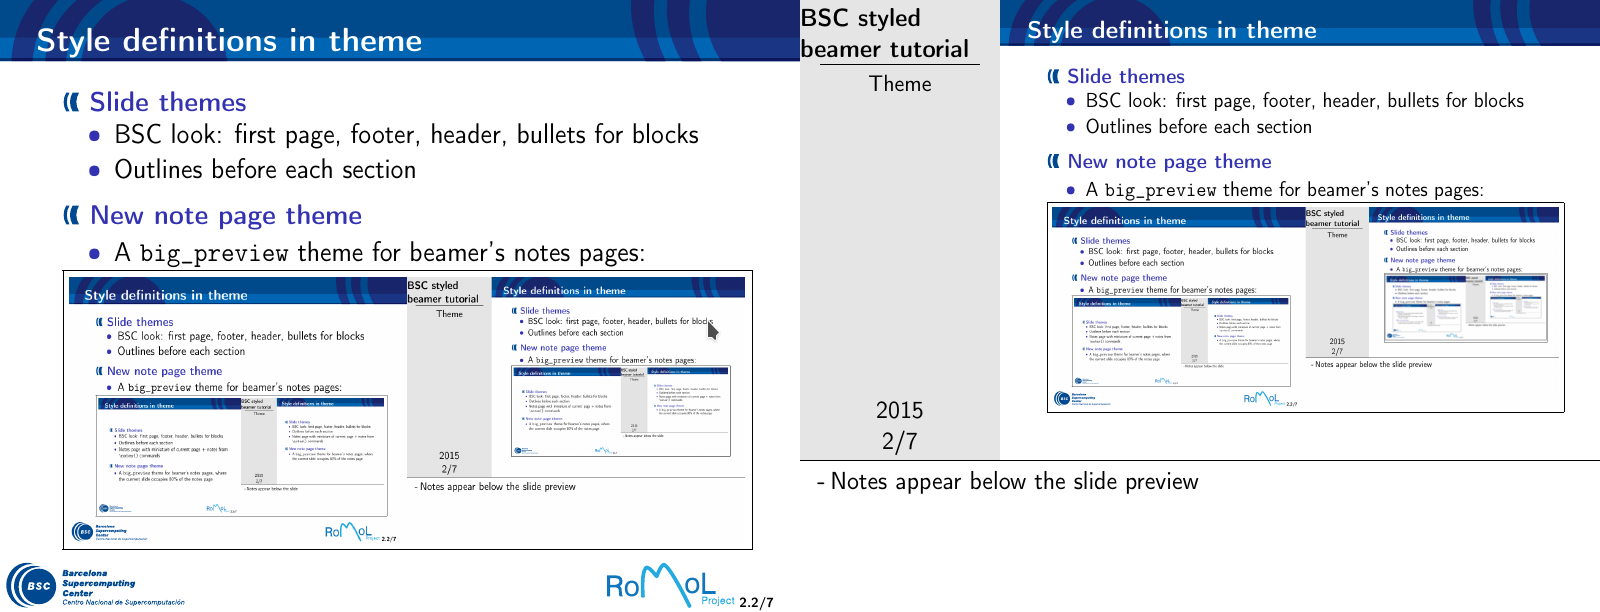
\includegraphics[width=.82\linewidth]{big_notes}}
		\end{center}
	\end{block}
\end{frame}

\begin{frame}[fragile]
	\frametitle{Command definitions}
	\begin{block}{New commands}
		\begin{itemize}
			\item the \verb|\notocsection| command, equivalent to \textbackslash section without outline before
			\item the \verb|\includesvg[optional width]{svg figure}| command, where the figure is given without the .svg extension, which includes a svg with latex-text inside
		\end{itemize}
	\end{block}
	\pause
	\begin{block}{Extended commands}
		\begin{itemize}
			\item the \verb|\appendix| command now stops slide numbering
		\end{itemize}
	\end{block}
\end{frame}

\begin{frame}[fragile]
	\frametitle{Bibliography}
	\begin{block}{You can cite as in any latex document}
		Citations integrate with the footnotes between the logos.
		\begin{itemize}
			\item Add a .bib file: \\ \verb|\addbibresource{bib file}|
			\item Set predefined style (before loading theme): \\ \verb|\PassOptionsToPackage{style=authortitle}{biblatex}|
			\item To use predefined style: \\ \verb|\cite{lamport94}|
			\item To put full citation in footnote\footfullcite{Lamport94}: \\ \verb|\footfullcite{Lamport94}|
			\item Same only on slide 2 of the frame: \\ \verb|\footnote<2>{\fullcite{Lamport94}}|
		\end{itemize}
	\end{block}
\end{frame}

\section{Makefile}

\begin{frame}[fragile]
	\frametitle[Makefile ft.]{Features in the Makefile}
	\begin{block}{Targets}
		\begin{itemize}
			\item{\textbf{by default}:} makes slides for all .tex files in directory
			\item{\textbf{notes}:} makes slides with content of \verb|\notes{}| commands on second screen.\\ Try opening with pympress for example.
			\item{\textbf{handout}:} 4 slides per page, no transitions
			\item{\textbf{clean}:} removes all generated files except .pdf
			\item{\textbf{allclean}:} removes all generated files
		\end{itemize}
	\end{block}
	\note{You won't see this in the normal presentation}
\end{frame}

\begin{frame}
	\frametitle{Figures}
	\begin{block}{svg files}
		\begin{itemize}
			\item requires inkscape
			\item Builds .pdf\_tex for every latex-text containing svg figure
			\item Builds .pdf for every other svg figure
		\end{itemize}
	\end{block}

	\begin{block}{On Windows}
		\begin{itemize}
			\item A script called \texttt{make\_figures\_on\_windows.bat} calls inkscape to export svg files to pdf / pdf\_tex
			\item Same behaviour as the Makefile on Linux
			\item Then just import the main.tex file in your \LaTeX editor
		\end{itemize}
	\end{block}
\end{frame}

\begin{frame}[fragile]
	\frametitle{Demonstrating file inclusion}
	\begin{block}{Here is a figure of some tasks being scheduled}
		It has some latex text content such as \verb|\alpha|
		\begin{figure}[h!]
		\centering
		\tiny % affects the font sizes in figure
		\includesvg[0.4\linewidth]{syntethictrace_async}
		\end{figure}
	\end{block}
	\vspace{-1em}\pause
	\begin{block}{The process of generating a TaskSim trace}
		\begin{columns}
		\begin{column}{0.3\linewidth}
			\begin{figure}[h!]
			\centering
			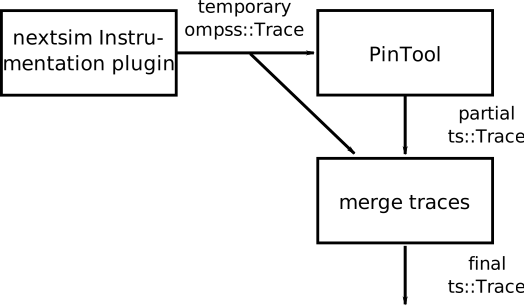
\includegraphics[width=\linewidth]{tracing_architecture}
			\end{figure}
		\end{column}
		\begin{column}{0.5\linewidth}
			This figure is just plain svg, so include a .pdf . Any other graphics format works as well (png, jpg, etc)
		\end{column}
		\end{columns}
	\end{block}
\end{frame}


\appendix

\begin{frame}
	\frametitle{This is a backup slide}
	\begin{block}{It appears after the \texttt{\textbackslash appendix} command}
		See how the bottom says ``Appx. A'' Instead of ``slide NN.N/NN''
	\end{block}
\end{frame}


\end{document}

